

\tikzset{every picture/.style={line width=0.75pt}} %set default line width to 0.75pt        

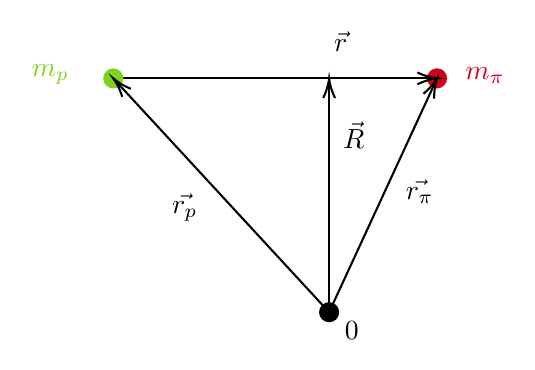
\begin{tikzpicture}[x=0.65pt,y=0.65pt,yscale=-1,xscale=1]
%uncomment if require: \path (0,300); %set diagram left start at 0, and has height of 300

%Flowchart: Connector [id:dp9827455772611288] 
\draw  [color={rgb, 255:red, 208; green, 2; blue, 27 }  ,draw opacity=1 ][fill={rgb, 255:red, 208; green, 2; blue, 27 }  ,fill opacity=1 ] (375,90) .. controls (375,87.24) and (377.24,85) .. (380,85) .. controls (382.76,85) and (385,87.24) .. (385,90) .. controls (385,92.76) and (382.76,95) .. (380,95) .. controls (377.24,95) and (375,92.76) .. (375,90) -- cycle ;
%Straight Lines [id:da5093684133345362] 
\draw    (200,90) -- (378,90) ;
\draw [shift={(380,90)}, rotate = 180] [color={rgb, 255:red, 0; green, 0; blue, 0 }  ][line width=0.75]    (10.93,-3.29) .. controls (6.95,-1.4) and (3.31,-0.3) .. (0,0) .. controls (3.31,0.3) and (6.95,1.4) .. (10.93,3.29)   ;
%Straight Lines [id:da04984112064582158] 
\draw    (320,220) -- (320,92) ;
\draw [shift={(320,90)}, rotate = 90] [color={rgb, 255:red, 0; green, 0; blue, 0 }  ][line width=0.75]    (10.93,-3.29) .. controls (6.95,-1.4) and (3.31,-0.3) .. (0,0) .. controls (3.31,0.3) and (6.95,1.4) .. (10.93,3.29)   ;
%Straight Lines [id:da13661676787341415] 
\draw    (320,220) -- (379.16,91.82) ;
\draw [shift={(380,90)}, rotate = 114.78] [color={rgb, 255:red, 0; green, 0; blue, 0 }  ][line width=0.75]    (10.93,-3.29) .. controls (6.95,-1.4) and (3.31,-0.3) .. (0,0) .. controls (3.31,0.3) and (6.95,1.4) .. (10.93,3.29)   ;
%Flowchart: Connector [id:dp37210275318157304] 
\draw  [color={rgb, 255:red, 126; green, 211; blue, 33 }  ,draw opacity=1 ][fill={rgb, 255:red, 126; green, 211; blue, 33 }  ,fill opacity=1 ] (195,90) .. controls (195,87.24) and (197.24,85) .. (200,85) .. controls (202.76,85) and (205,87.24) .. (205,90) .. controls (205,92.76) and (202.76,95) .. (200,95) .. controls (197.24,95) and (195,92.76) .. (195,90) -- cycle ;
%Straight Lines [id:da8769015497622031] 
\draw    (320,220) -- (201.36,91.47) ;
\draw [shift={(200,90)}, rotate = 47.29] [color={rgb, 255:red, 0; green, 0; blue, 0 }  ][line width=0.75]    (10.93,-3.29) .. controls (6.95,-1.4) and (3.31,-0.3) .. (0,0) .. controls (3.31,0.3) and (6.95,1.4) .. (10.93,3.29)   ;
%Flowchart: Connector [id:dp5562170943538245] 
\draw  [color={rgb, 255:red, 0; green, 0; blue, 0 }  ,draw opacity=1 ][fill={rgb, 255:red, 0; green, 0; blue, 0 }  ,fill opacity=1 ] (315,220) .. controls (315,217.24) and (317.24,215) .. (320,215) .. controls (322.76,215) and (325,217.24) .. (325,220) .. controls (325,222.76) and (322.76,225) .. (320,225) .. controls (317.24,225) and (315,222.76) .. (315,220) -- cycle ;

% Text Node
\draw (153,80.4) node [anchor=north west][inner sep=0.75pt]  [color={rgb, 255:red, 126; green, 211; blue, 33 }  ,opacity=1 ]  {$m_{p}$};
% Text Node
\draw (394,82.4) node [anchor=north west][inner sep=0.75pt]  [color={rgb, 255:red, 208; green, 2; blue, 27 }  ,opacity=1 ]  {$m_{\pi }$};
% Text Node
\draw (326,112.4) node [anchor=north west][inner sep=0.75pt]    {$\vec{R}$};
% Text Node
\draw (361,144.4) node [anchor=north west][inner sep=0.75pt]    {$\vec{r_{\pi }}$};
% Text Node
\draw (231,152.4) node [anchor=north west][inner sep=0.75pt]    {$\vec{r_{p}}$};
% Text Node
\draw (321,62.4) node [anchor=north west][inner sep=0.75pt]    {$\vec{r}$};
% Text Node
\draw (327,223.4) node [anchor=north west][inner sep=0.75pt]    {$0$};


\end{tikzpicture}